%!TEX root = Manuscrit.tex
\chapter{Jeux de données en télédétection}
\label{chap:datasets}
%\subsection{Jeux de données en télédétection}

Il existe plusieurs jeux de données pour la classification d'images optiques de télédétection. Citons ainsi les jeux de données \emph{UC Merced}~\cite{yang_bag--visual-words_2010} contenant 2 100 images aériennes dans 21 classes d'occupation des sols, \emph{Brazilian Coffe}~\cite{penatti_deep_2015} d'images \gls{SPOT} pour la classification de terrains cultivés et SAT-4/SAT-6~\cite{basu_deepsat_2015} contenant respectivement 500 000 et 405 000 images aériennes pour plusieurs classes d'occupation des sols. L'inconvénient de ces jeux de données est d'une part la faible taille des images (256$\times$\SI{256}{\px} pour \emph{UC Merced} et \emph{Brazilian Coffe}, 28$\times$\SI{28}{\px} pour SAT) et la faible quantité d'annotations. En effet, ces jeux de données, prévus pour la classification, ne peuvent que difficilement être utilisés pour la segmentation sémantique. Cependant, plusieurs jeux de données comprenant des annotations denses ont été proposés.

\section{ISPRS 2D Semantic Labeling}
\label{annexe:isprs}

\begin{figure}[h]
		%\foreach\picid in {7,21,28}{%
		\foreach\picid in {7,28}{%
		\begin{subfigure}{0.33\textwidth}
			\includegraphics[angle=90,width=\textwidth]{vaihingen_top_\picid}
			\caption*{Image RVB}
		\end{subfigure}%
		\begin{subfigure}{0.33\textwidth}
			\includegraphics[angle=90,width=\textwidth]{vaihingen_ndsm_\picid}
			\caption*{\gls{MNH}}
		\end{subfigure}%
		\begin{subfigure}{0.33\textwidth}
			\includegraphics[angle=90,width=\textwidth]{vaihingen_gt_\picid}
			\caption*{Vérité terrain}
		\end{subfigure}
		}
    \caption{Images ortho-rectifiées et \gls{MNH} pour le jeu de données \gls{ISPRS} Vaihingen .}
    \label{fig:isprs_vaihingen}
\end{figure}

\begin{figure}[h]
		\foreach\picid in {3_10,6_11}{%7_12}{%
		\begin{subfigure}{0.33\textwidth}
			\includegraphics[width=\textwidth]{potsdam_top_\picid}
			\caption*{Image RVB}
		\end{subfigure}%
		\begin{subfigure}{0.33\textwidth}
			\includegraphics[width=\textwidth]{potsdam_ndsm_\picid}
			\caption*{\gls{MNH}}
		\end{subfigure}%
		\begin{subfigure}{0.33\textwidth}
			\includegraphics[width=\textwidth]{potsdam_gt_\picid}
			\caption*{Vérité terrain}
		\end{subfigure}
		}
	\caption{Images ortho-rectifiées et \gls{MNH} pour le jeu de données \gls{ISPRS} Potsdam.}
	\label{fig:isprs_potsdam}
\end{figure}

Le jeu de données \glssymbol{ISPRS} 2D Semantic Labeling~\cite{rottensteiner_isprs_2012} est constitué de deux ensembles d'images aériennes \glsfirst{THR} fournies par le groupe de travail WG II/4 de l'\glsdesc{ISPRS}. Dans les deux cas, il s'agit de scènes urbaines disposant de cinq classes d'intérêt pour la segmentation sémantique\,: surfaces imperméables (routes, parkings, trottoirs\dots), bâtiments, végétation basse, arbres et véhicules. Une classe de rejet est également définie et comprend le mobilier urbain (bancs, poubelles, conteneurs\dots) et les surfaces inclassables (terrains de basketball, zones en travaux, points d'eau\dots).

Le jeu de données se décline en deux scènes. La première est issue d'une acquisition aéroportée sur la ville de Vaihingen (Allemagne) et comporte une mosaïque de 33 tuiles \gls{IRRV} ortho-rectifiées à une résolution de \SI{9}{\centi\meter/\px}. L'acquisition optique est accompagnée d'une acquisition \gls{Lidar} à la même résolution, dont a été extrait un \gls{MNE}. Un \gls{MNH} pré-calculé~\cite{gerke_use_2015} dérivé du \gls{MNE} est également disponible. Les ortho-images sont fournies en format \gls{TIFF} encodés sur 8 bits, tandis que le \gls{MNE} est fourni en flottant sur 32 bits. Toutes les données ont été recalées sur la même grille de pixels. Les images ont une taille moyenne d'environ $2600\times1900$px, soit une surface d'approximativement $40 000m^2$. Vaihingen est une ville de taille moyenne (28 853 habitants en 2009), caractérisée par une urbanisation moyenne composée majoritairement de pavillons résidentiels et d'espace verts urbains.

La seconde scène est une acquisition aéroportée sur la ville de Potsdam (Allemagne) et comporte une mosaïque de 38 tuiles \gls{IRRVB} à une résolution de \SI{5}{\centi\meter/\px} réalisée par BSF Swissphoto. Le jeu de données est fourni par la \emph{Deutsche Gesellschaft für Photogrammetrie, Fernerkundung und Geoinformation} (DGPF)\footnote{\url{http://www.ifp.uni-stuttgart.de/dgpf/DKEP-Allg.html}}. Les tuiles présentent toutes les mêmes dimensions, à savoir $6000\times6000$px, soit une surface de \SI{90 000}{\meter\squared}. Un \gls{MNE} et un \gls{MNH} dérivé sont également fournis. Des annotations denses sont disponibles pour les mêmes classes que précédemment sur 24 images. À nouveau, l'ensemble des modalités sont recalées sur la même grille de pixels et les images sont fournies en \gls{TIFF} sur 8 bits, tandis que les modèles de surface sont fournis en flottant sur 32 bits. Potsdam est une ville urbanisée relativement grande (161 468 habitants en 2013), caractérisée par de nombreux immeubles, un réseau routier dense. À noter la présence d'un canal et de nombreux travaux de construction à la date de l'acquisition des images.

Quelques exemples représentatifs des deux acquisitions sont montrés dans les~\cref{fig:isprs_vaihingen,fig:isprs_potsdam}. Le nombre de pixels dans chaque classe est détaillé dans la~\cref{fig:isprs_barplots}.

Les images dont les annotations ne sont pas rendues publiques servent à évaluer en aveugle les méthodes proposées par la communauté. La commission WG II/4 de l' \gls{ISPRS} gère ainsi un tableau de résultat public\footnote{\url{http://www2.isprs.org/commissions/comm2/wg4/vaihingen-2d-semantic-labeling-contest.html}}\footnote{\url{http://www2.isprs.org/commissions/comm2/wg4/potsdam-2d-semantic-labeling.html}}, détaillant les performances obtenues par différentes méthodes de l'état-de-l'art.

\section{Data Fusion Contest 2015}
\label{annexe:dfc2015}

\begin{figure}[h]
		\foreach\picid in {1,2}{%
		\begin{subfigure}{0.33\textwidth}
			\includegraphics[width=\textwidth]{dfc2015_top\picid}
			\caption*{Image RVB}
		\end{subfigure}%
		\begin{subfigure}{0.33\textwidth}
			\includegraphics[width=\textwidth]{dfc2015_dsm\picid}
			\caption*{\gls{MNH}}
		\end{subfigure}%
		\begin{subfigure}{0.33\textwidth}
			\includegraphics[width=\textwidth]{dfc2015_gt\picid}
			\caption*{Vérité terrain}
		\end{subfigure}
		}
	\caption{Images ortho-rectifiées et \gls{MNH} pour le jeu de données \glssymbol{DFC} 2015.}
	\label{fig:dfc2015}
\end{figure}

Le jeu de données \gls{DFC} 2015~\cite{campos-taberner_processing_2016} est issu d'une compétition de fusion de données organisée par le groupe de travail \gls{GRSS} de l'\gls{IEEE}. Ce jeu de données comporte une mosaïque de 7 images couleurs ortho-rectifiées de dimensions $10 000\times10 000$ à une résolution au sol de \SI{5}{\centi\meter/\px}, soit une surface par tuile de \SI{250 000}{\meter\squared}. L'acquisition a été réalisée sur la zone portuaire de Zeebruges (Belgique) en mars 2011 par le département Communication, Information, Systèmes \& Senseurs (CISS) de l'École royale militaire de Belgique. Il est accompagné d'une acquisition \gls{Lidar} comprenant environ \SI{65}{points/\meter\squared} espacés chacun de \SI{10}{\centi\meter}. Les données couleurs sont fournies en \gls{TIFF} encodé sur 8 bits et les données \gls{Lidar} sont fournis rastérisées sous la forme d'un \gls{MNE} en flottant sur 32 bits, ainsi qu'un nuage de points. Il s'agit d'une scène principalement urbaine présentant principalement des installations portuaires.

 Des annotations denses ont été réalisées par l'\gls{ONERA}~\cite{lagrange_benchmarking_2015} pour les classes bateau, voiture, végétation basse, arbre, bâtiment, eau et surface imperméable. La~\cref{fig:dfc2015} montre quelques exemples d'images extraites du jeu de données et la~\cref{fig:dfc2015_barplot} détaille la répartition des pixels dans les différentes classes.

Un tableau de résultats public est maintenu par l'\gls{IEEE} \gls{GRSS}\footnote{\url{http://dase.ticinumaerospace.com/}} afin de permettre la comparaison entre différentes méthodes de classification.

\section{Data Fusion Contest 2018}
\label{annexe:dfc2018}

\begin{figure}[h]
  \begin{subfigure}{\textwidth}
    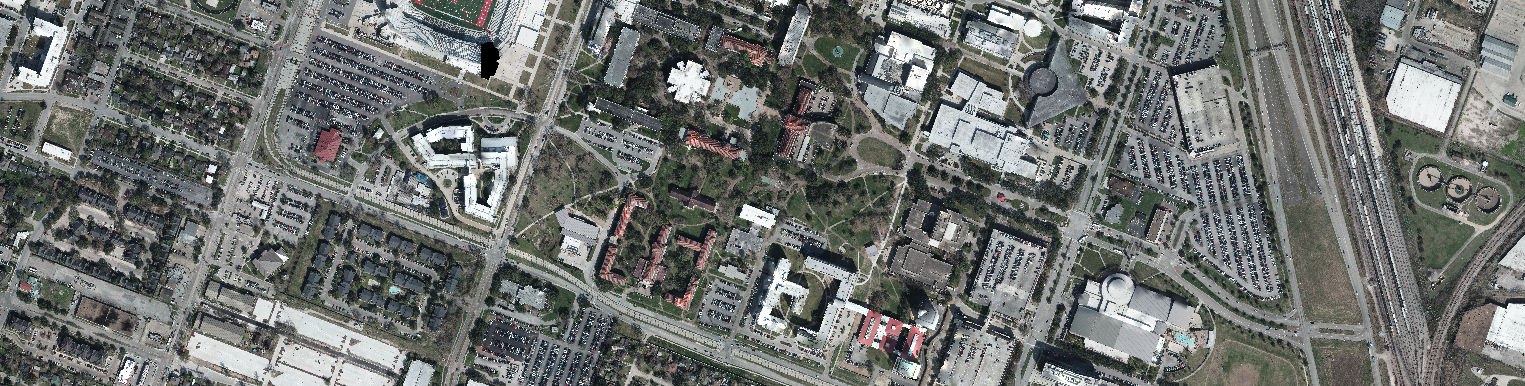
\includegraphics[width=\textwidth]{dfc2018_top}
    \caption{Image \gls{RVB}}
  \end{subfigure}
  \begin{subfigure}{\textwidth}
    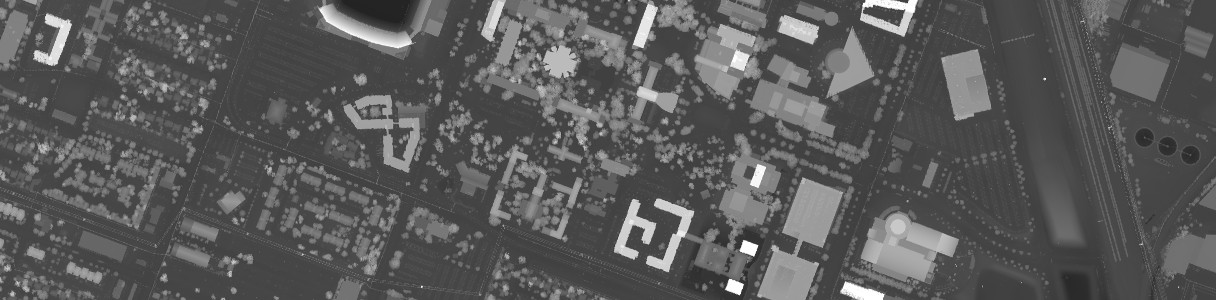
\includegraphics[width=\textwidth]{dfc2018_dsm}
    \caption{\gls{MNH}}
  \end{subfigure}
  \begin{subfigure}{\textwidth}
    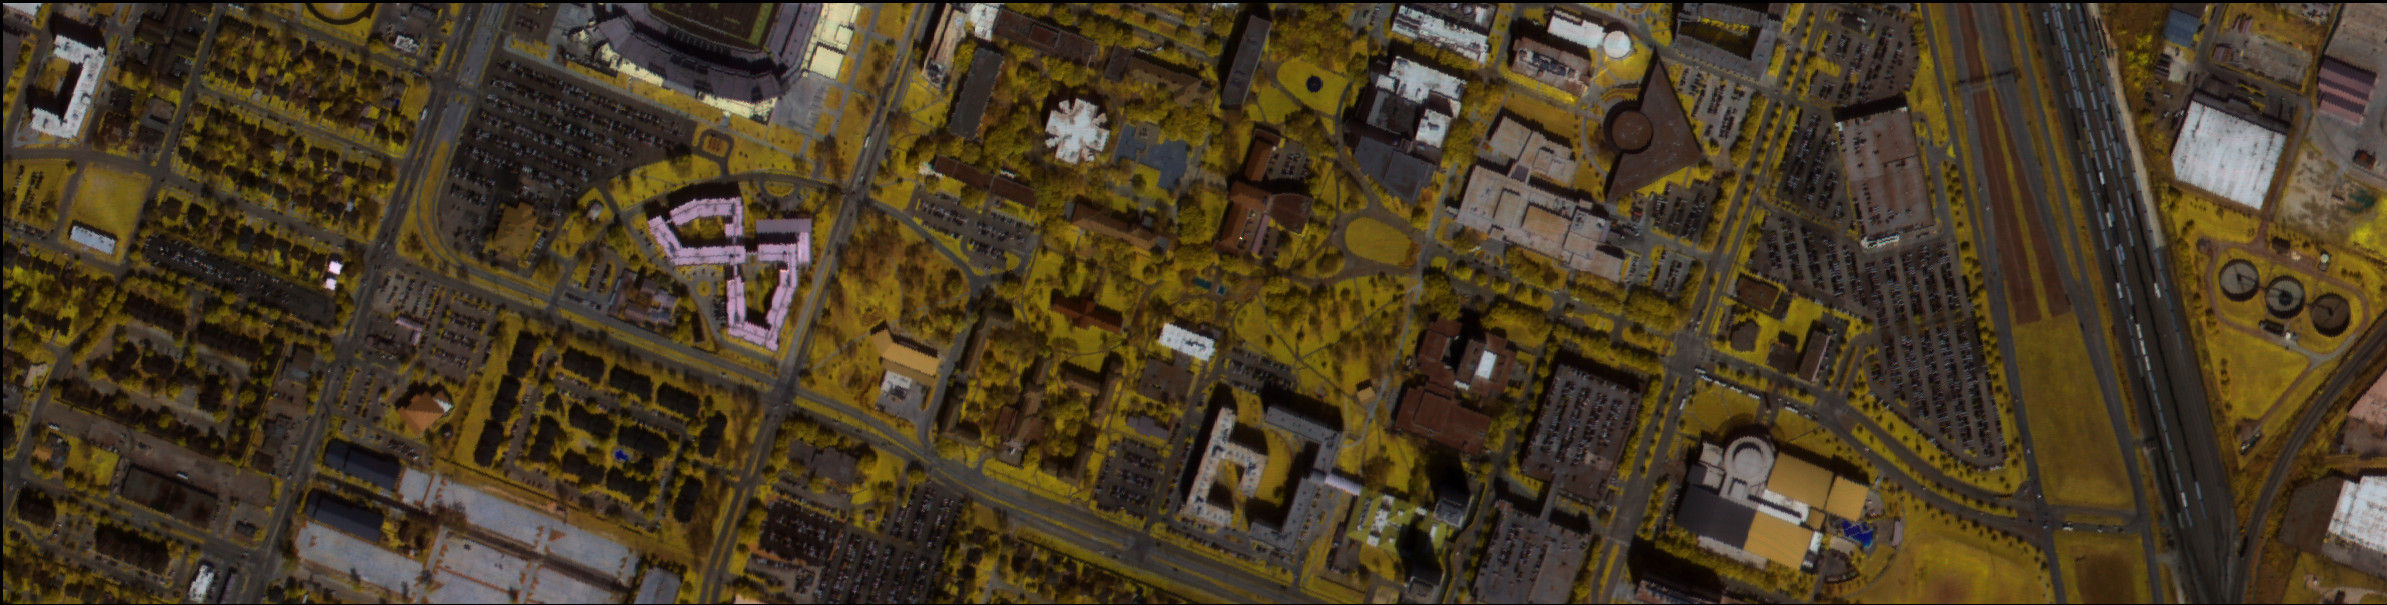
\includegraphics[width=\textwidth]{dfc2018_hsi}
    \caption{Image hyperspectrale (fausses couleurs)}
  \end{subfigure}
  \begin{subfigure}{\textwidth}
    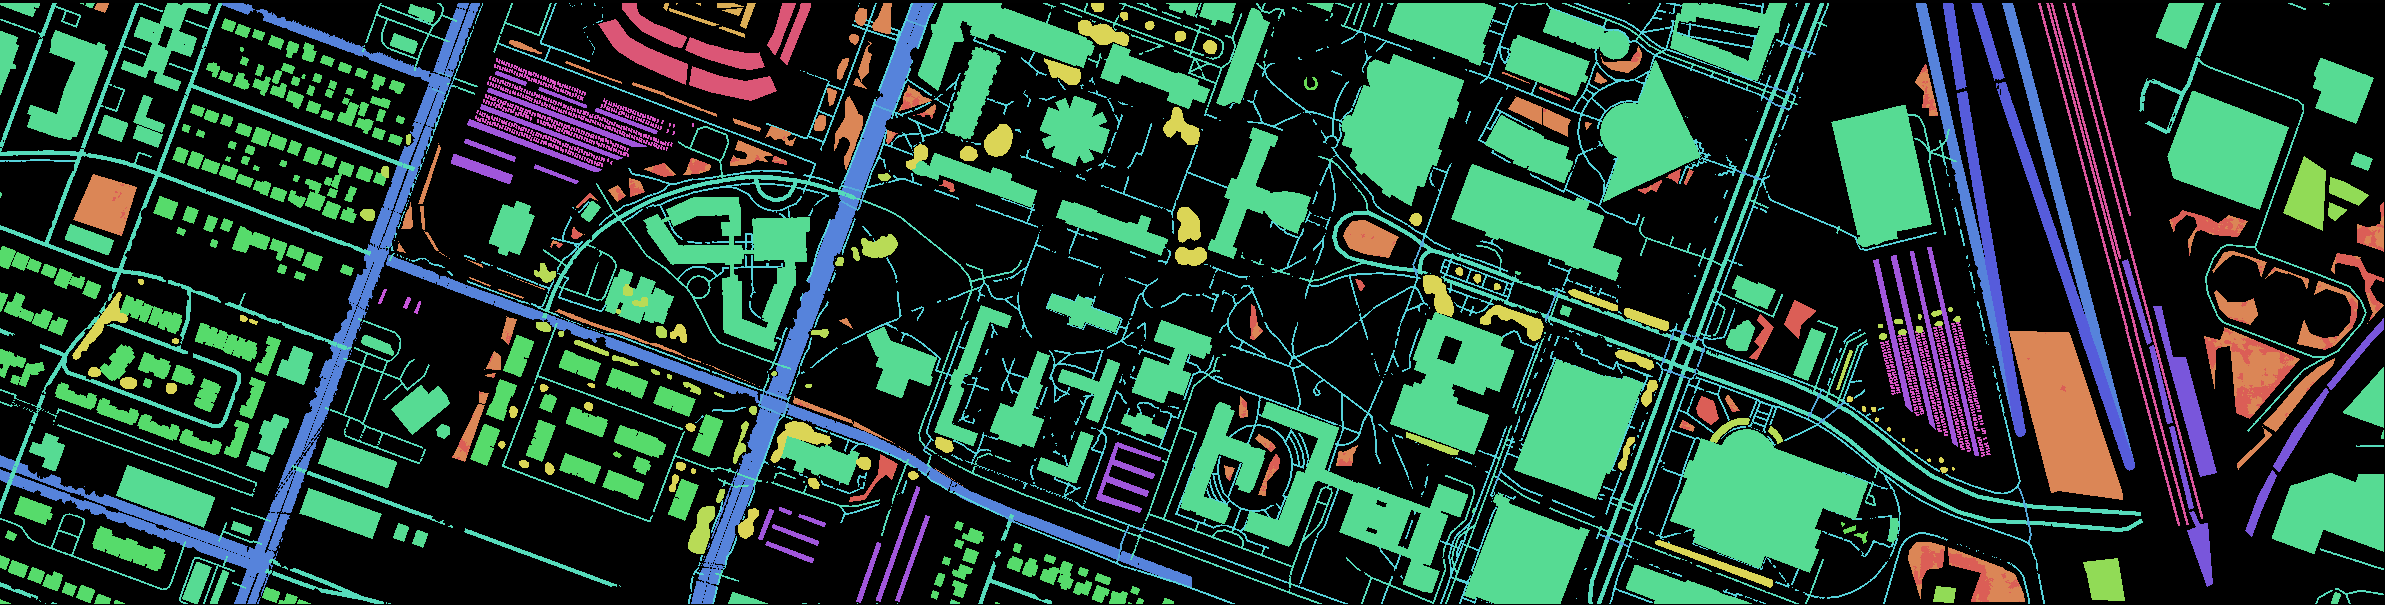
\includegraphics[width=\textwidth]{dfc2018_gt}
    \caption{Vérité terrain}
  \end{subfigure}
  \caption{Données d'entraînement du concours \gls{DFC} 2018.}
  \label{fig:dfc2018}
\end{figure}

Le jeu de données \gls{DFC} 2018~\cite{le_saux_2018_2018} est également issu de la compétition \glsfirst{DFC} organisée par l'\gls{IEEE} \gls{GRSS}. Il comporte 14 images aériennes \gls{RVB} ortho-rectifiées \gls{THR} à \SI{5}{\centi\meter/\px} de dimensions $12000\times12000$, accompagnées par une image hyperspectrale à 48 bandes à \SI{1}{\meter/\px} entre 380 et \SI{1050}{\nano\meter}. Une acquisition \gls{Lidar} multispectrale est également disponible à une résolution de \SI{0,5}{\meter/\px}, dont est dérivé un \gls{MNH}. L'ensembles des données sont géoréférencées et recalées. Les données ont été acquises par le \emph{National Center for Airborne Laser Mapping} sur la ville de Houston (États-Unis) en février 2017.
L'image concerne principalement l'université de Houston et ses alentours, par conséquent il s'agit d'une scène très urbanisée incluant des installations massives (gare et voies de chemins de fer, stade). Des annotations partielles sont fournies pour la moitié du jeu de données sur diverses classes d'intérêt urbaines, l'autre moitié des annotations étant conservées secrètes pour l'évaluation.
Le jeu d'apprentissage est illustré par la~\cref{fig:dfc2018}  et la~\cref{fig:dfc2018_barplot} détaille la répartition des pixels dans les différentes classes.

Un tableau de résultats public est maintenu par l'\gls{IEEE} \gls{GRSS}\footnote{\url{http://dase.ticinumaerospace.com/}} afin de permettre la comparaison entre différentes méthodes de classification.

\section{Inria Aerial Image Labeling}
\label{annexe:inria}

\begin{figure}[h]
  \foreach \picpath\picname in {chicago5_top/Ortho-image (Chicago),chicago5_gt/Vérité terrain (Chicago),vienna2_top/Ortho-image (Vienne),vienna2_gt/Vérité terrain (Vienne)}{%
  \begin{subfigure}[t]{0.25\textwidth}%
    \includegraphics[width=\textwidth]{\picpath}%
    \caption*{\picname}
  \end{subfigure}%
  }
  \caption{Exemples d'images extraites de la base de données \emph{Inria Aerial Image Labeling}.}
  \label{fig:inria}
\end{figure}

Le jeu de données \emph{Inria Aerial Image Labeling}~\cite{maggiori_can_2017} contient 360 images \gls{RVB} ortho-rectifiées de taille $5000\times5000$px à une résolution de \SI{30}{\centi\meter/\px}, soit une surface de \SI{2,25}{\kilo\meter\squared}. Les images ont été compilées depuis les bases de données de l'USGS pour Austin, Chicago, Kitsap County, Bellingham, Bloomington et San Francisco et depuis les services géographiques régionaux autrichiens pour le Tyrol, Vienne et Innsbruck. Il s'agit d'acquisitions aéroportées, ortho-rectifiées, ré-échantillonnée à \SI{30}{\centi\meter/\px} et fournies sous un format couleur 8 bits. Les annotations des empreintes de bâtiments sont obtenues à partir des sources cadastrales locales. La moitié des images peuvent être utilisées pour l'entraînement de modèles d'extraction de bâtiments, les annotations étant disponibles librement. Le reste du jeu de données est réservé à l'évaluation des modèles par les auteurs du jeu de données. Quelques images et annotations du jeu d'apprentissage sont illustrées dans la~\cref{fig:inria}.

Parmi ces villes, plusieurs sont de grandes agglomérations caractérisées par une forte densité de bâtiments, mêlant habitations personnelles, constructions massives (gares, hôpitaux, usines\dots) et immeubles. À l'inverse, les autres zones présentent une densité de bâtiments modérée voire faible, avec un relief et une végétation importants pour le Tyrol. Cette diversité des profils de zones observées vise à permettre de mesurer la capacité des modèles à généraliser à différents environnements géographiques.

Les organisateurs gèrent un tableau de résultats public\footnote{\url{https://project.inria.fr/aerialimagelabeling/leaderboard/}} permettant de comparer les performances obtenues par différentes méthodes.

\section{NZAM/ONERA Christchurch}
\label{annexe:christchurch}

\begin{figure}[h]
	\foreach \picnum in {1,2,3,4}{%
	\begin{subfigure}{0.5\textwidth}
		\includegraphics[width=\textwidth]{christchurch_gt_\picnum}
	\end{subfigure}%
	\ifthenelse{\equal{\picnum}{2}}{\\}{}%
	}%
	\caption{Images et annotations extraites du jeu de données NZAM/ONERA Christchurch.}
	\label{fig:christchurch}
\end{figure}

Le jeu de données NZAM/ONERA Christchurch comporte 4 images \gls{RVB} ortho-rectifiées à une résolution de \SI{10}{\centi\meter/\px} acquises après la séisme ayant frappé la ville de Christchurch en Nouvelle-Zélande le 22 février 2011. Les images sont distribuées sous licence Creative Commons Attribution 3.0 par le \emph{New Zealand's Land Information Office}~\footnote{\url{http://www.linz.govt.nz/land/maps/linz-topographic-maps/imagery-orthophotos/christchurch-earthquake-imagery}}. Chaque image, de dimensions $\approx 5000\times4000$, a été annotée par l'ONERA/DTIS~\cite{randrianarivo_urban_2013} pour les classes d'intérêt ``bâtiments'' (797 objets), ``véhicules'' (2 357 objets) et ``végétation'' (938 objets). L'ensemble des objets sont annotées par une boîte englobante polygonale, ce qui en fait des annotations moins précises que les vérité terrain pixelliques des jeux de données \gls{ISPRS}, par exemple. Des exemples sont données dans la~\cref{fig:christchurch}.

\section{VEDAI}
\label{annexe:vedai}

\begin{figure}[h]
	\foreach\picnum in {15,30,43}{%
		\begin{subfigure}{0.32\textwidth}
			\includegraphics[width=\textwidth]{vedai_000000\picnum}
		\end{subfigure}
	}
	\caption{Extraits d'images annotées du jeu de données VEDAI.}
	\label{fig:vedai}
\end{figure}

La base de données VEDAI (\emph{Vehicle Detection in Aerial Imagery})~\cite{razakarivony_vehicle_2016} est une collection d'images aériennes ortho-rectifiées mises à disposition par l'\emph{Automated Geographic Reference Center} de l'Utah. Les images, acquises au printemps 2012, ont une résolution au sol de \SI{12,5}{\centi\meter/\px} et comportent 4 canaux, \gls{RVB} et infrarouge, encodés sur 8 bits. Les images originales ont été découpées en 1 210 tuiles de dimensions $1 024\times 1 024$. Une version sous-échantillonnée à \SI{25}{\centi\meter/\px} utilisant des tuiles de dimensions $512\times512$ est également disponible.

Les véhicules présents dans les images sont annotés à fin de détection par des boîtes englobantes ainsi qu'une étiquette correspondant au type de véhicule. Neuf classes d'intérêt sont ainsi identifiées\,: avion, bateau, camping-car, voiture, pick-up, tracteur, camion, van et une classe ``autres''. Les coordonnées du centre du véhicule et l'angle correspondant à son orientation principale sont également annotés.

Ce jeu de données couvre des zones principalement rurales avec une faible densité de véhicules. Les images présentent une large variété de contextes, comme des parkings, des aérodromes, des axes routiers plus ou moins importants, des champs et des habitations. Quelques exemples d'images et d'annotations correspondantes sont montrés dans la~\cref{fig:vedai}.

\section{CamVid}
\label{annexe:camvid}

\begin{figure}[h]
	\foreach \picnum in {1,2,3}{%
		\includegraphics[width=0.32\textwidth]{camvid_rgb_\picnum}
	}\\
	\foreach \picnum in {1,2,3}{%
		\includegraphics[width=0.32\textwidth]{camvid_gt_\picnum}
	}\\
	\caption{Images \gls{RVB} (première ligne) et annotations pixelliques (deuxième ligne) extraites du jeu de données CamVid.}
	\label{fig:camvid}
\end{figure}

La base de données CamVid (\emph{Cambridge-driving Labeled Video Database})~\cite{brostow_semantic_2009} est une collection d'images extraite à \SI{1}{\hertz} d'une vidéo \gls{RVB} de 10 minutes en situation de conduite automobile dans la ville de Cambridge (Royaume-Uni). 367 images d'entraînement et 233 images de test à une résolution de $360\times480$ ont été extraites des vidéos et manuellement annotées dans 11 classes d'intérêt telles que la route, les bâtiments, les autres véhicules, les piétons, les panneaux de signalisations, le trottoir, etc. Dans l'ensemble, il s'agit d'images embarquées de conduite à vitesse réduite dans un environnement urbain comprenant de nombreux objets mobiles.

La~\cref{fig:camvid} montre quelques exemples d'images annotées du jeu d'entraînement.

\section{SUN RGB-D}
\label{annexe:sun}

\begin{figure}[h]
	\foreach\picnum in {10097,05320,06370}{%
	\includegraphics[width=0.32\textwidth]{\picnum}
	\includegraphics[width=0.32\textwidth]{\picnum_depth}
	\includegraphics[width=0.32\textwidth]{\picnum_labels}\\
	}%
	\caption{Images \gls{RVB}, carte de profondeur et annotations extraites du jeu de donneés SUN RGB-D.}
	\label{fig:sunrgbd}
\end{figure}

Le jeu de données SUN RGB-D~\cite{song_sun_2015} comporte 10 335 images \glsdesc{RGB-D} d'intérieur acquises en utilisant plusieurs capteurs (Kinect, Xtion, RealSense). Chaque image est une paire couleur \gls{RVB} et carte de profondeur et a été annotée au niveau pixel pour 37 classes d'intérêt d'objets ou de surfaces telles que ``chaise'', ``sol'', ``mur'' ou encore ``table''. Les images sont généralement redimensionnées à $224\times224$. En tout, 146 617 objets 2D sont annotés sous forme de polygones non recouvrants, permettant ainsi d'obtenir pour chaque scène une vérité terrain de segmentation sémantique. D'autres annotations sont également disponibles comme la catégorie de la scène 2,5D parmi les 47 disponibles ou 800 types d'objets 3D identifiés par une boîte englobante.

Des exemples d'images \glssymbol{RGB-D} et d'annotations sont données dans la~\cref{fig:sunrgbd}.

\begin{figure}[h]
	\begin{subfigure}{0.5\textwidth}
		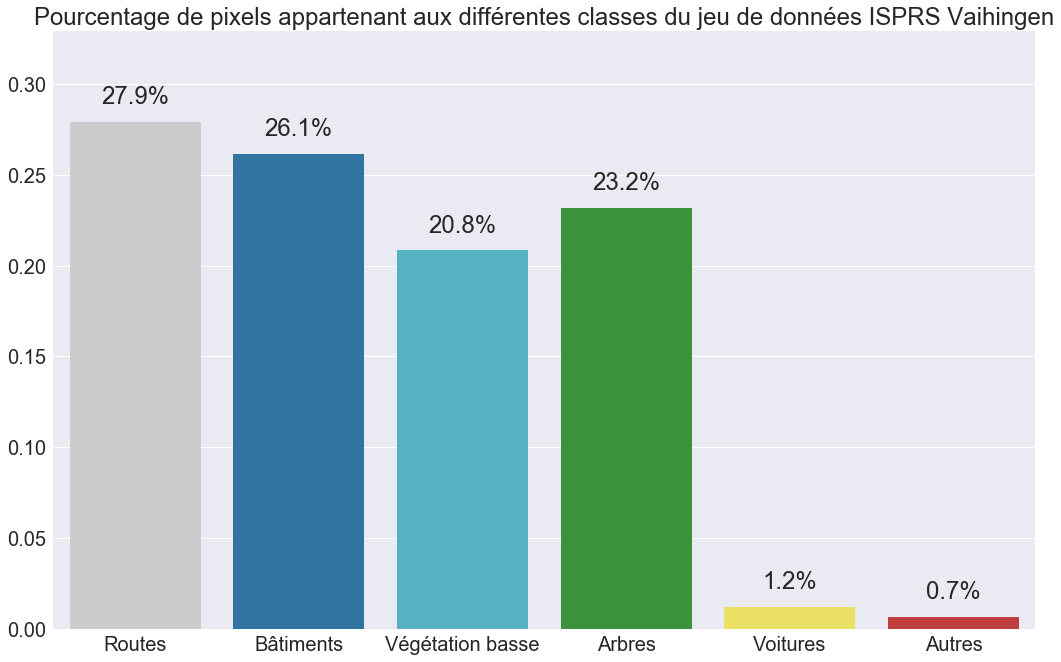
\includegraphics[width=\textwidth]{vaihingen_barplot}
	\end{subfigure}
	\begin{subfigure}{0.5\textwidth}
		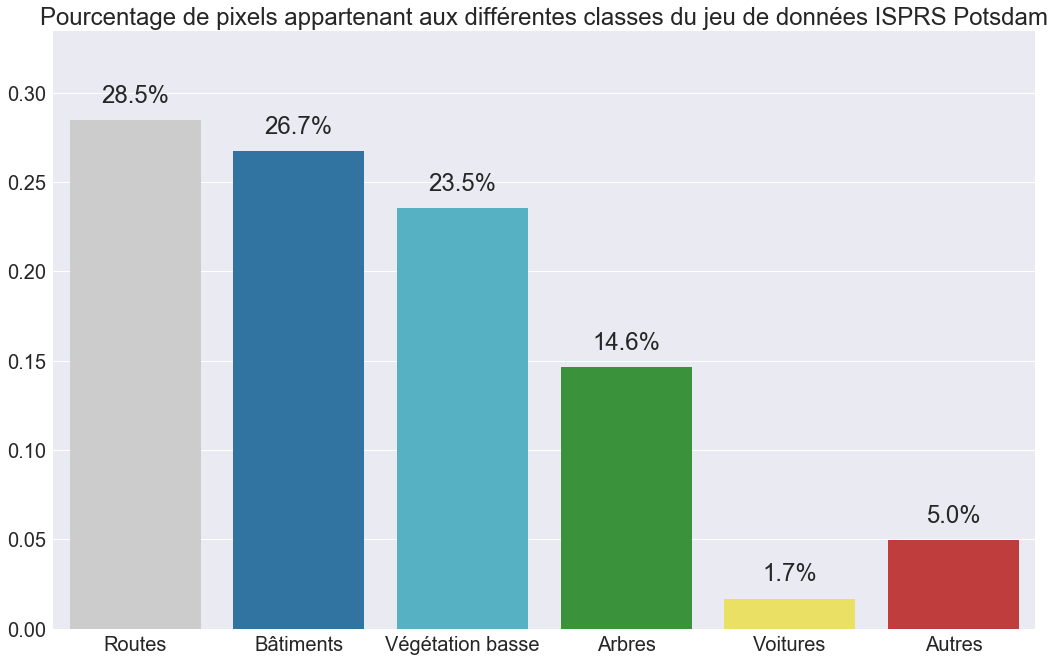
\includegraphics[width=\textwidth]{potsdam_barplot}
	\end{subfigure}
	\caption{Répartition des pixels des jeux de données \gls{ISPRS} dans différentes classes d'intérêt.}
	\label{fig:isprs_barplots}
\end{figure}


\begin{figure}[h]
	\begin{subfigure}[t]{0.5\textwidth}
		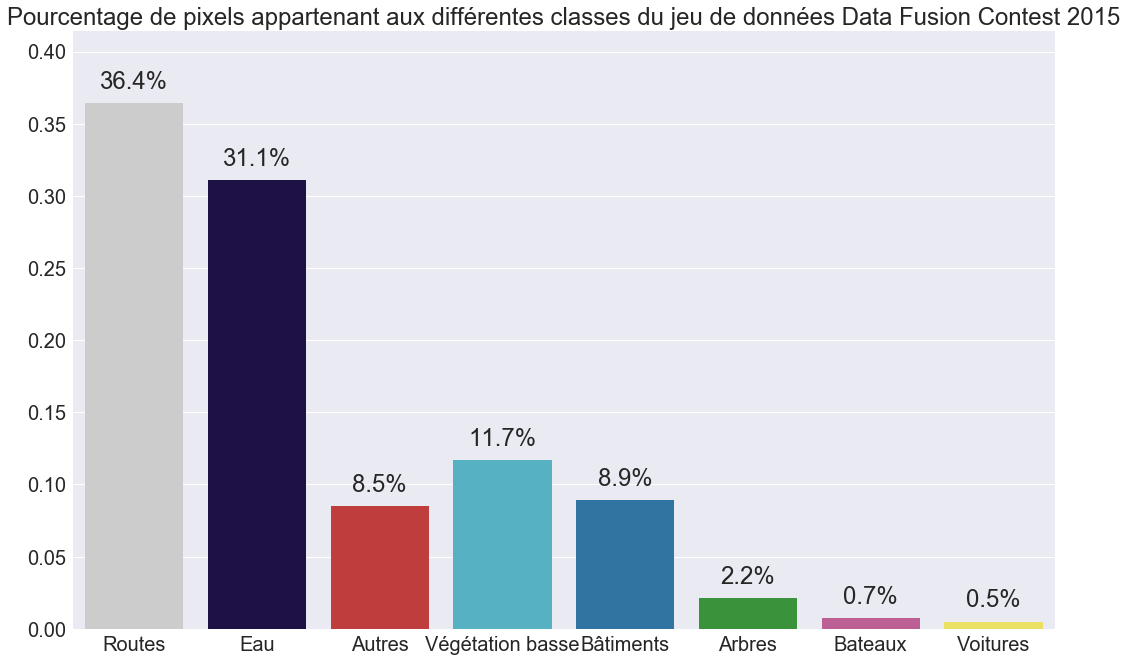
\includegraphics[width=\textwidth]{dfc2015_barplot}
		\caption{Répartition des pixels du jeu de données \glssymbol{DFC} 2015.}
		\label{fig:dfc2015_barplot}
	\end{subfigure}
	\begin{subfigure}[t]{0.5\textwidth}
		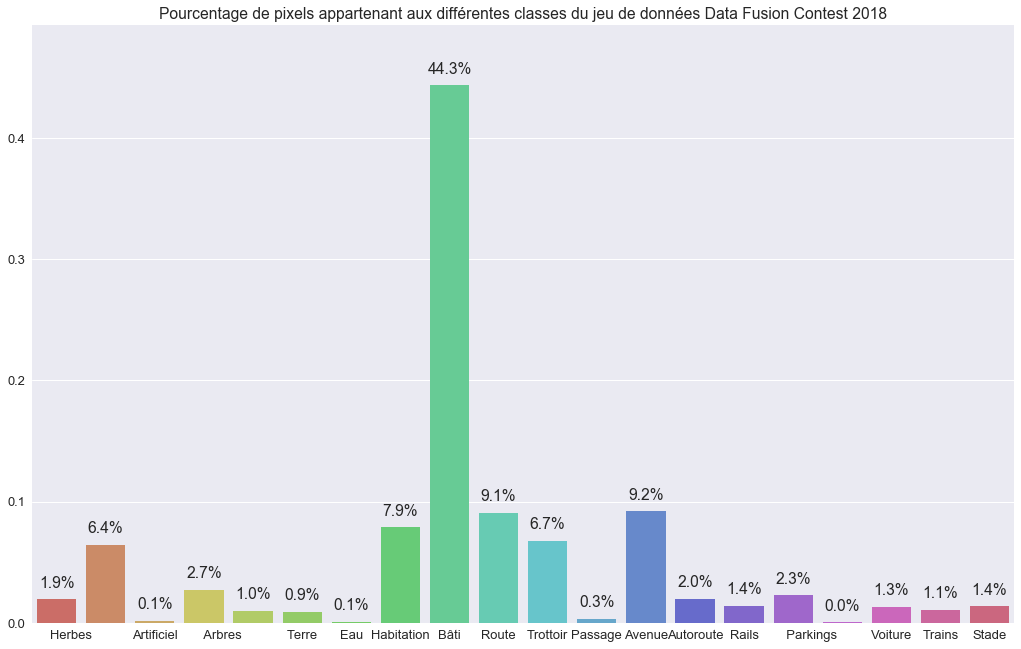
\includegraphics[width=\textwidth]{dfc2018_barplot}
		\caption{Répartition des pixels du jeu de données \glssymbol{DFC} 2018.}
		\label{fig:dfc2018_barplot}
	\end{subfigure}
\end{figure}

\begin{figure}[h]
	\begin{subfigure}{0.5\textwidth}
		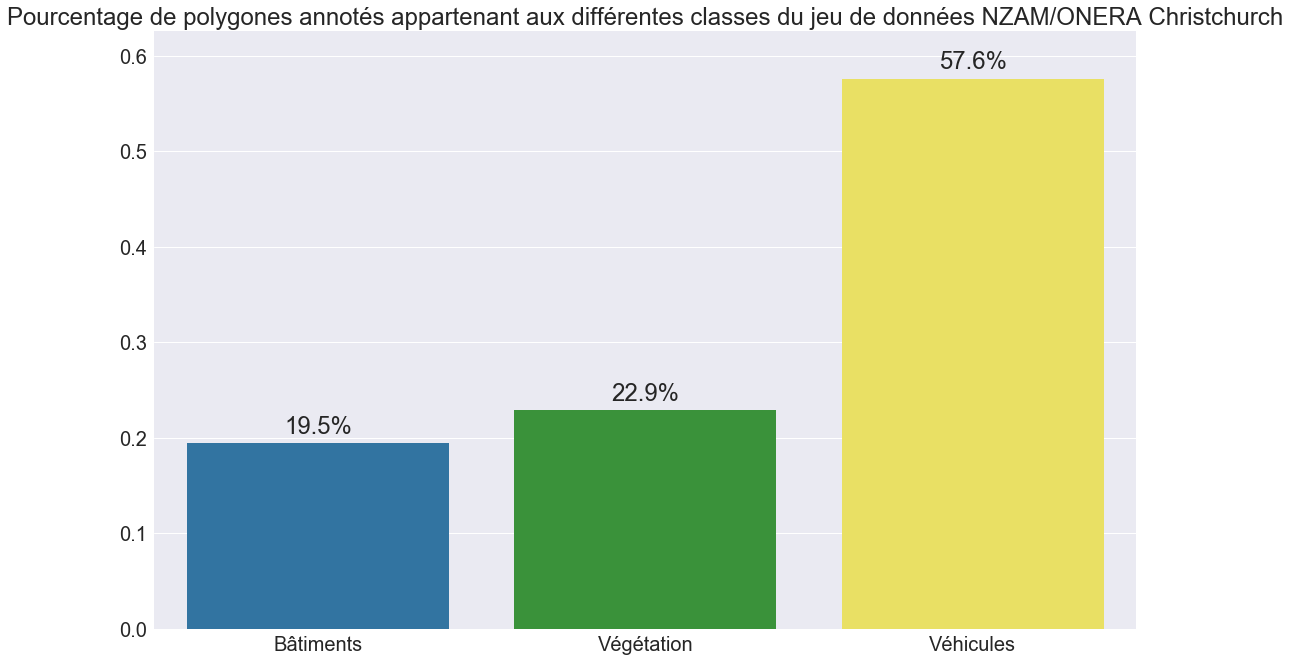
\includegraphics[width=\textwidth]{christchurch_barplot_polygons}
	\end{subfigure}
	\begin{subfigure}{0.5\textwidth}
		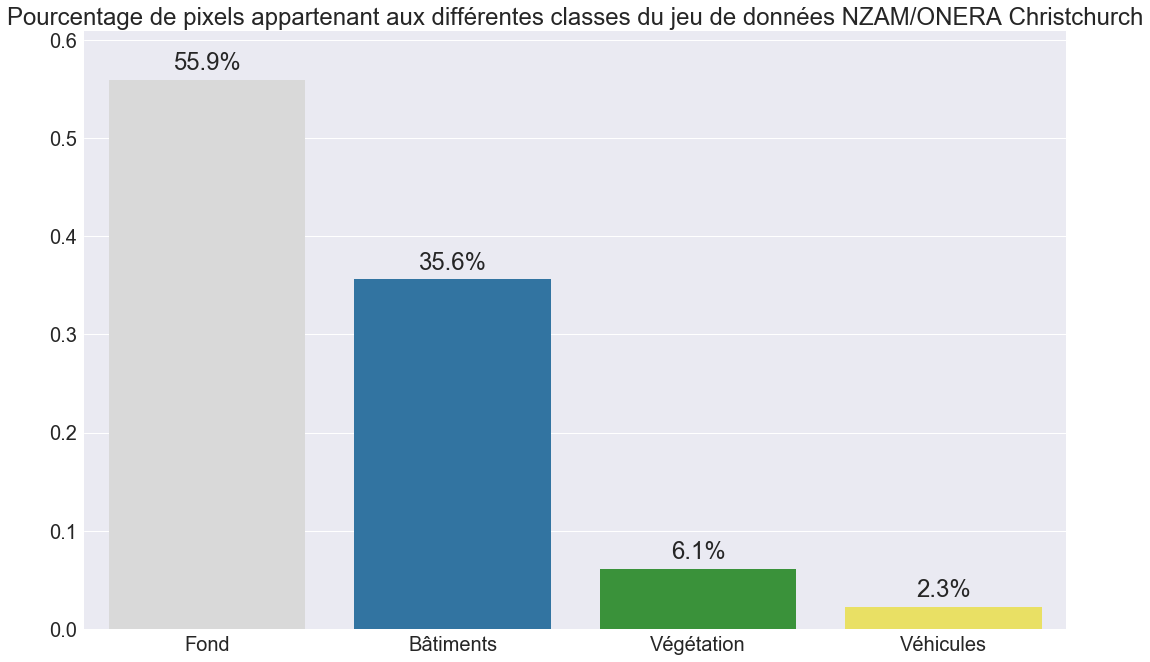
\includegraphics[width=\textwidth]{christchurch_barplot_pixels}
	\end{subfigure}
\end{figure}

\bibliographystyle{plainnat}
\bibliography{Annexes/Datasets}
